\section{Introduction}
\label{sec:intro}
Deep neural networks (DNNs) have made remarkable progress across various domains by delivering superior performance on large-scale datasets. However, while the benefits of training DNNs on large-scale datasets are undeniable, these algorithms also tend to inadvertently acquire unwanted biases \cite{NEURIPS2020_6cfe0e61}, hampering their generalization. For instance, a classifier predominantly trained to recognize camels in desert landscapes could encounter difficulties when attempting to identify a camel situated on a road \cite{Kim_2021_ICCV}. While a certain degree of bias can enhance model performance, as exemplified by the assumption that cars usually travel on roads \cite{Choi_2020_CVPR}, it remains critical to identify and address unwanted biases. 
% \begin{figure}
%     \centering
%     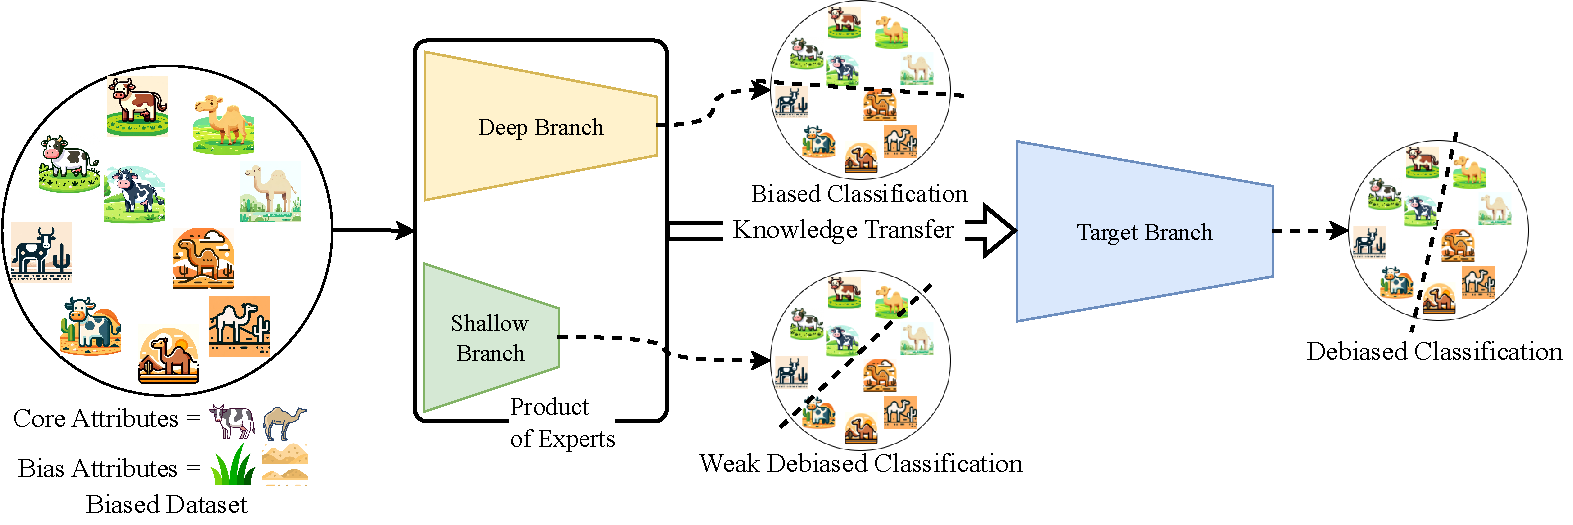
\includegraphics[width=\textwidth]{figures/teaser_diagram.pdf}
%     \caption{Our DeNetDM model comprises a Product of Expert (PoE) \cite{Hinton:02}, featuring one deep and one shallow expert. The shallow expert primarily captures core attributes, achieving debiased classification, while the deep expert focuses on bias. To compensate for the shallow expert's limited capability due to less depth, we implement a knowledge transfer strategy utilizing knowledge from the experts to train a target debiased model.}
%     \label{fig:teaser-diagram}
% \end{figure}
Previous methods to address this problem rely on bias annotations as suggested in \cite{9607491,Kim_2019_CVPR,sagawa2019distributionally,wang2020fair}, and may involve predefined bias types, such as texture bias mitigation approach in \cite{geirhos2018imagenettrained}. 
% . For instance, in \cite{geirhos2018imagenettrained}, texture bias is mitigated by training a shape-oriented classifier using augmented data and style transfer. However, this approach limits the ability of models to achieve robustness against biases for which obtaining prior knowledge is a challenging endeavor. 
However, acquiring bias labels with human resources is expensive and time-consuming. Recent studies, including \cite{NEURIPS2020_eddc3427} and \cite{NEURIPS2021_disentangled},  have shifted towards debiasing methods without bias labels, with approaches like \cite{NEURIPS2020_eddc3427} emphasizing bias-aligned samples and reweighting bias-conflicting samples, while others like \cite{NEURIPS2021_disentangled,Kim_2021_ICCV} introduce augmentation strategies to diversify bias-conflicting points.

We propose DeNetDM (\textbf{De}biasing by \textbf{Net}work \textbf{D}epth \textbf{M}odulation), a novel approach to automatically identify and mitigate spurious correlations in image classifiers without relying on explicit data augmentation or reweighting. We start by showing that a sample set that exhibits bias through spurious correlation of attributes lies on a manifold with an effective dimensionality (rank) lower than its bias-free counterpart.
% We then leverage this finding to formally derive a relationship between the depth of a network and the true rank of the attribute (not sample) subspace that it learns and generalizes to.
We then leverage this finding to formally derive a relationship between the depth of a network and the true rank of the attribute (not sample) subspace that it encodes. We find for a set of attributes that are equally likely to minimize the empirical risk, a deeper network prefers to retain those with a lower rank, with a higher probability. This implies that the depth of a network acts as an implicit regularizer in the rank space of the attributes.
We find that deeper networks tend to generalize based on bias attributes and shallower networks tend to generalize based on core attributes. This finding is in line with a number of works that show that deeper networks tend to learn low rank solutions in general \citep{roy2007effrank, huh2023simplicitybias, wang2024implicit}.
% Note, however, that previous works make no claim about the relationship between the depth of a network and the attribute subspace that it generalizes to, a link we establish in our work for the first time, to the best of our knowledge.
Note, however that prior works do not establish the relationship between network depth and the rank of the attribute subspace, a link we establish in our work for the first time, to the best of our knowledge.

Our theoretical claims are confirmed by our preliminary empirical study on linear feature decodability, which quantifies the extent to which specific data attributes can be accurately and reliably extracted from a given dataset or signal. Our study focuses on the feature decodability of bias and core attributes in the neural networks of varying depths, following the approach outlined in \cite{NEURIPS2020_71e9c662}. Our observations in untrained neural networks reveal that the feature decodability tends to diminish as the networks become deeper. We also investigate how attribute decodability varies with Empirical Risk Minimization (ERM) based training on networks of varying depths. 
% A detailed discussion of the experiment can be found in \cref{sec:linear_decodability_analysis}.


% DeNetDM is based on insights gained from our preliminary study on feature decodability, which quantifies the extent to which specific data attributes can be accurately and reliably extracted from a given dataset or signal. Our study focuses on the feature decodability of bias and core attributes in the neural networks of varying depths, following the approach outlined in \cite{NEURIPS2020_71e9c662}. Our observations in untrained neural networks reveal that the feature decodability tends to diminish as the networks become deeper. We also investigate how attribute decodability varies with Empirical Risk Minimization (ERM) based training on networks of varying depths. A detailed discussion of the experiment can be found in \cref{sec:linear_decodability_analysis}.
% We conduct a brief experiment to analyze the feature decodability, specifically focusing on bias and core attributes, using untrained neural networks of different depths, following the approach outlined in \cite{NEURIPS2020_71e9c662}. Our observations reveal that the attribute decodability tends to diminish as the neural networks becomes deeper. Additionally, we investigate the variation in attribute decodability when employing Empirical Risk Minimization (ERM) based training on networks of different depths. These experiments yield interesting results that form the foundation of our proposed approach DeNetDM. A detailed discussion of the experimental setting and the conclusions can be found in \cref{sec:linear_decodability_analysis}. 
% We eliminate the necessity for explicit reweighting or augmentation of bias-conflicting data points by employing a novel approach based on a simple observation, which entails modulating the depth of a pair of neural networks.

% \abhra{
% SUGGESTED REWRITE FOR THE LAST PARAGRAPH:
% We start by showing that a sample set that exhibits bias through spurious correlation of attributes lies on a manifold with an effective dimensionality (rank) lower than its bias-free counterpart. We then leverage this finding to formally derive a relationship between the depth of a network and the true rank of the attribute (not sample) subspace that it learns and generalizes to. We find that deeper networks tend to generalize based on bias attributes and shallower networks tend to generalize based on core attributes. This finding is in line with a number works that show that deeper networks tend to learn low rank solutions in general \citep{roy2007effrank, huh2023simplicitybias, wang2024implicit}. Note, however, that previous works make no claim about the relationship between the depth of a network and the attribute subspace that it generalizes to, a link we establish in our work for the first time, to the best of our knowledge.
% }
Our hypothesis posits that in a task requiring deep and shallow branches to acquire distinct information, the deep branch consistently prioritizes bias attributes, while the shallow branch favors core attributes. We utilize a technique inspired by the Product of Experts \citep{Hinton:02}, where one expert is deeper than the other. Empirical analysis shows that the deep branch becomes perfectly biased and the shallow branch becomes relatively debiased by focusing solely on the core attributes by the end of the training. Since the shallow branch may lack the capacity to capture the nuances of the core attributes adequately due to less depth, we propose a strategy where we train a deep debiased model utilizing the information acquired from both deep (perfectly biased) and shallow (weak debiased) network in the previous phase. Our training paradigm efficiently facilitates the learning of core attributes from bias-conflicting data points to the debiased model of any desired architecture. 

In summary, we make the following contributions: (1) We theoretically prove that the deep models prefer to learn spurious correlations compared to shallower ones, supported by empirical analysis of the decodability of bias and core attributes across neural networks of varying depths. (2) Building upon the insights from our decodability experiments, we present a novel debiasing approach that involves training both deep and shallow networks to obtain a desired debiased model. (3) We perform extensive experiments and ablation studies on a diverse set of datasets, including synthetic datasets like Colored MNIST and Corrupted CIFAR-10, as well as real-world datasets, Biased FFHQ, BAR and CelebA, demonstrating an approximate 5\% improvement over existing methods.
    % \item Our results demonstrate that our approach outperforms existing state-of-the-art methods, with an approximate 5\% performance improvement.


